\documentclass[12pt,a4paper]{article}
\usepackage{graphicx}
\usepackage[left=2cm, right=2cm, top=2cm]{geometry}
\begin{document}
\paragraph{}
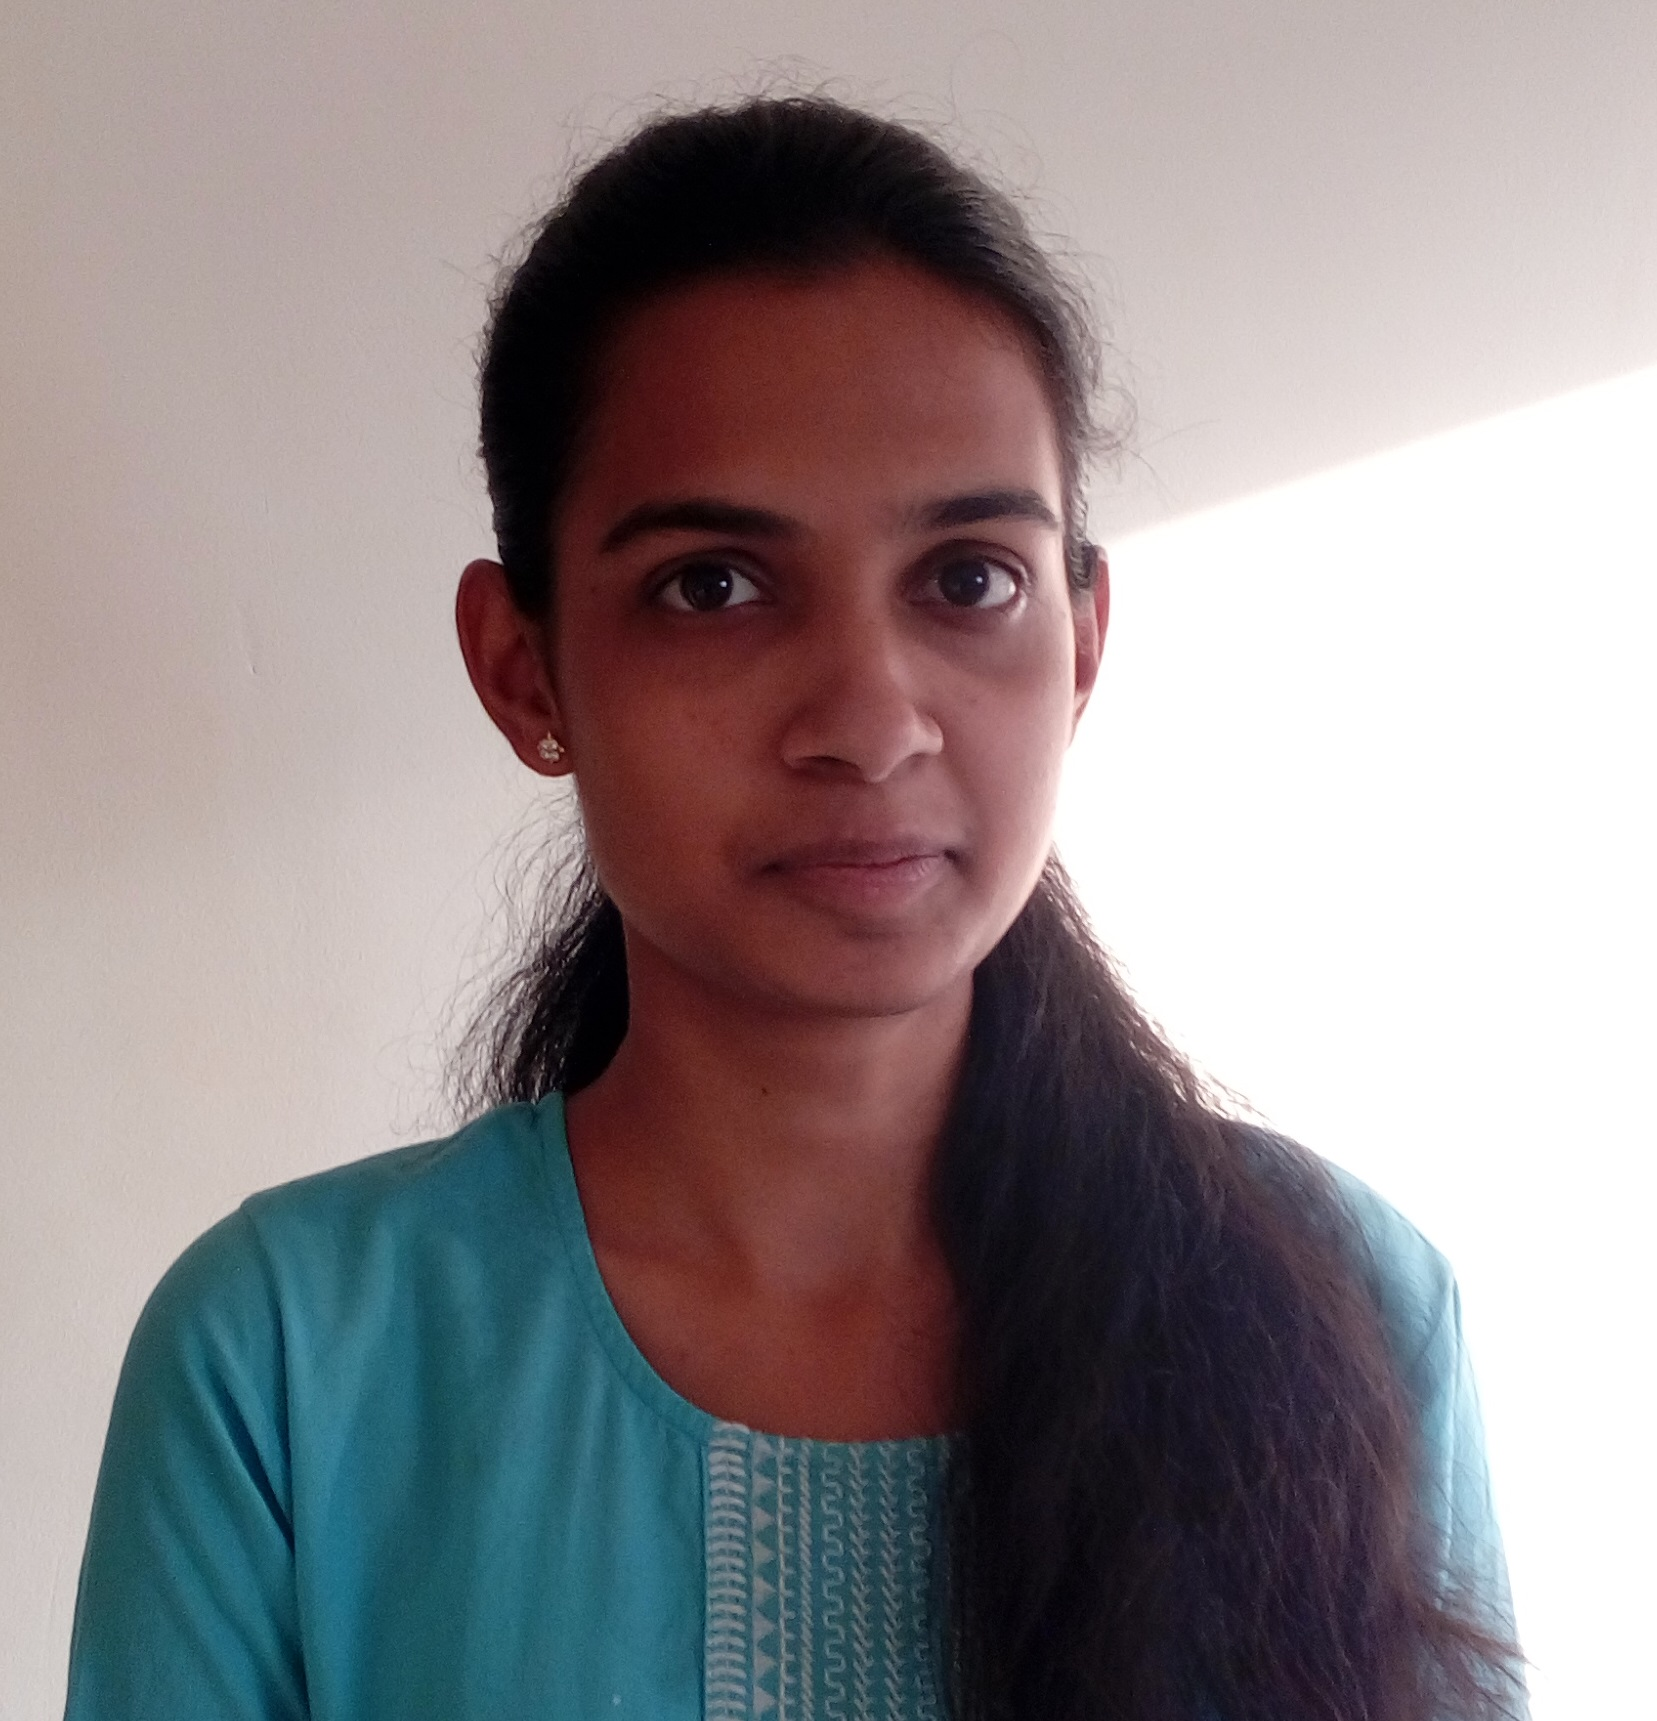
\includegraphics[scale=0.05]{profile}
\textbf{\LARGE Supriya Mane\\}\hfill
\\
\mbox{E-mail ID:\large supriya9597@gmail.com}\\
\mbox{Contact no:\large +91 7022900515}\\
\mbox{\large KLS GIT, Belagavi}\\
\paragraph{OBJECTIVE}
\line(1,0){400}\\
My goal is to pursue a career as an Electronics and Communication engineer in Embedded systems domain. Currently, I am looking for an internship where I can learn under professional guidance and also provide some inputs to the organization according to my skills.
\paragraph{EDUCATION}
	\line(1,0){400}
	\begin{itemize}
  		\item \textrm{X}(Secondary)\\
  			Year of Completion: 2013\\
			GOA BOARD OF SECONDARY AND HIGHER SECONDARY EDUCATION(St.Joseph's Institue)\\
			Percent: 91.8\verb"%"
  		\item \textrm{XII}(Higher Secondary)
  			Year of Completion: 2015\\
			GOA BOARD OF SECONDARY AND HIGHER SECONDARY EDUCATION(Mushtifund Higher Secondary School)\\
			Percent: 81.8\verb"%"
  		\item Bachelor of Engineering(B.E), Electronics and Communications(2015-2019)\\
  			  KLS Gogte Institute Of Technology\\
			  CGPA : 8.52/10(5th sem)
	\end{itemize}
\paragraph{PROJECTS}
	\line(1,0){420}
	\begin{itemize}
		\item \verb"[Current]Encryption techniques for IoT"
		\begin{itemize}
			\item Study of lightweight cryptography algorithms for IoT
			\item Implementing for TI Cc2650 or Cc2640R2F boards
			\item Comparing their performance with standard AES
		\end{itemize}
		\item Collector Bot-A bot that collects Fresh fruits avoiding damaged fruits and drop in Truck. It involved following components:
		\begin{itemize}
			\item A completely designed bot for moving and picking and dropping fruits
			\item Truck(Spark V)
			\item Use of ArUco Markers for simulation in Virtual Robot Experimentation Platform
			\item Python+VREP at Supervisor station to control Collector bot using Xbee\\
		\end{itemize}
	\end{itemize}
\paragraph{TRAINING/INTERNSHIP}
	\line(1,0){320}
	\begin{itemize}
		\item Hardware Descriptive Language,  IEEE (Online) during Apr 2017 - Aug 2017\\
Online training of hardware design using verilog.
	\item Arduino Workshop at KLS Gogte Institute Of Technology (Belgaum) in May 2016\\
A two-day workshop on Arduino Nano board to understand the basics
	\item Internet of Things workshop at KLS Gogte Institute of Technology in August 2016.
	\item Internship at Galaxy Machinery Pvt Ltd (Belagavi) in Design Electrical Department during July 2017 for 2 weeks.
	\end{itemize}
\paragraph{RESEARCH PUBLICATIONS}
	\line(1,0){300}
	\begin{itemize}
		\item None
	\end{itemize}

\paragraph{TECHNICAL SKILLS}
	\line(1,0){350}
	\begin{itemize}
		\item C Programming
		\item ARM Microcontroller
		\item Python
		\item Matlab
		\item HDL-Verilog
	\end{itemize}
\paragraph{SOFT SKILLS}
	\line(1,0){390}
	\begin{itemize}
		\item Leadership
		\item Work ethics
		\item Interpersonal
		\item Teamwork
	\end{itemize}
\paragraph{EXTRA-CURRICULAR ACTIVITIES}
	\line(1,0){270}
	\begin{itemize}
		\item Master Leader at LEaders Accelerating Development(LEAD), a program of Deshpande Foundation
		\item Volunteer at Yuva Summit'16, Annual Flagship International Conference held at Hubballi
	\end{itemize}
\paragraph{CO-CURRICULAR ACTIVITIES}
	\line(1,0){270}
	\begin{itemize}
		\item Participated in eYantra Robotics Competition 2016 organized by IIT Bombay
		\item Won 2nd place at eYantra Robotics Competition 2017 organized by IIT Bombay
		\item Coordinator at annual college technical fest Avalanche'17
	\end{itemize}
\paragraph{PERSONAL DETAILS}
	\line(1,0){350}
	\begin{itemize}
		\item Father's Name: Vishwas Mane
		\item Mother's Name: Sujata Mane
		\item Sex: Female
		\item Date of Birth: 09th May 1997
		\item Nationality: Indian
		\item Marital Status: Single
	\end{itemize}
\paragraph{REFERENCE}
	\line(1,0){400}
	\begin{itemize}
		\item Roopa Kulkarni\\
		Assistant Professor, KLS Gogte Institute of Technology\\
		Email-ID: rrkulkarni@git.edu\\
		Contact No: 0831-2498505
		\item Sagar Santaji\\
		Assistant Professor, KLS Gogte Institute of Technology\\
		Email-ID: sssantaji@git.edu\\
		Contact No: 0831-2498505
		
	\end{itemize}
\paragraph{DECLARATION}
	\line(1,0){380}\\
	I hereby declare that all the details provided are true to the best of my knowledge
\paragraph{DATE}
	\line(1,0){440}\\
	\em\today

\end{document}